% =====================================================================
%  PROGRESS REPORT  (Group Flower)  --  compile with XeLaTeX
%  Overleaf: Menu -> Compiler -> XeLaTeX, and upload the fonts/ folder
%  (Noto Sans Thai, SIL Open Font License) next to main.tex.
%  Figures in figures/ are generated by make_figures.py from the saved
%  result CSVs in baselines/cache/.
% =====================================================================
\documentclass[12pt]{report}

\usepackage{fontspec}
\usepackage{amsmath,amssymb}
\usepackage{natbib}
\usepackage[hidelinks]{hyperref}
\usepackage[left=1.5in,right=1in,top=1in,bottom=1in]{geometry}
\usepackage{graphicx}
\usepackage{setspace}
\usepackage{titlesec}
\usepackage{placeins}
\usepackage{longtable}
\usepackage{float}
\usepackage{booktabs}
\usepackage{tabularx}
\usepackage{array}
\usepackage{xcolor}
\usepackage{enumitem}
\usepackage[font=small,labelfont=bf]{caption}

% --- Thai script (only used inside \thai{...}) ---
\newfontfamily\thaifont{NotoSansThai-Regular.ttf}[Path=fonts/, BoldFont=NotoSansThai-Bold.ttf, Script=Thai, Scale=0.92]
% Switch to the Thai font automatically for characters U+0E00--U+0E7F only, so spaces,
% digits and punctuation inside Thai text keep the main font (Noto Sans Thai has no Latin).
\newXeTeXintercharclass\thaiclass
\count255="0E00
\loop \XeTeXcharclass\count255=\thaiclass \ifnum\count255<"0E7F \advance\count255 by 1 \repeat
\XeTeXinterchartokenstate=1
\XeTeXinterchartoks 0 \thaiclass = {\begingroup\thaifont}
\XeTeXinterchartoks 4095 \thaiclass = {\begingroup\thaifont}
\XeTeXinterchartoks \thaiclass 0 = {\endgroup}
\XeTeXinterchartoks \thaiclass 4095 = {\endgroup}
\newcommand{\thai}[1]{#1}
% Thai has no spaces between words: let ICU find line-break points
\XeTeXlinebreaklocale "th"
\XeTeXlinebreakskip = 0pt plus 1pt

\onehalfspacing

\titleformat{\chapter}[display]
  {\centering\bfseries}
  {\MakeUppercase{\chaptertitlename} \thechapter}
  {6pt}
  {\centering\Large\bfseries\MakeUppercase}
\titlespacing*{\chapter}{0pt}{0pt}{24pt}

\setcitestyle{authoryear,round}
\renewcommand{\arraystretch}{1.2}
\newcolumntype{L}{>{\raggedright\arraybackslash}X}
\newcommand{\status}[1]{\textbf{#1}}
\setlist{itemsep=2pt,topsep=4pt}

\begin{document}

% =====================================================================
%  TITLE PAGE
% =====================================================================
\begin{titlepage}
\singlespacing
\begin{center}
\vspace*{1.2cm}
\begin{spacing}{1.5}
{\LARGE \textbf{EXPLAINABLE REVIEWED-ITEM RETRIEVAL, WITH A THAI TASTE CASE STUDY}}
\end{spacing}

\vspace{0.6cm}
{\large Progress Report}

\vspace{0.4cm}
{\small (Proposal title: \emph{Explainable Reviewed-Item Retrieval: Searching Restaurants by Taste Preference})}

\vspace{2.0cm}
by

\vspace{0.5cm}
{\large Chidsanuphong Pengchai (st127004)}\\[6pt]
{\large Samichi Rungta (st127012)}

\vspace{1.5cm}
Group: Flower

\vspace{2.2cm}
Asian Institute of Technology\\
Department of Data Science and Artificial Intelligence\\
Thailand

\vspace{1cm}
October 19, 2026
\end{center}
\end{titlepage}

\singlespacing
\tableofcontents
\listoffigures
\listoftables
\onehalfspacing
\clearpage

% =====================================================================
%  CHAPTER 1: FEEDBACK SUMMARY
% =====================================================================
\chapter{Response to Proposal Feedback}
\label{ch:feedback}

\section{Feedback Summary Page}

Table~\ref{tab:feedback} answers every comment received on the proposal. Each row states
what we understood the comment to mean, what we did, and where the evidence is. Detailed
answers follow in Sections~\ref{sec:f1}--\ref{sec:fq}.

{\singlespacing\small
\begin{longtable}{@{}p{2.9cm}p{3.6cm}p{5.4cm}p{2.1cm}@{}}
\caption{Feedback summary: one row per comment from the proposal presentation.}
\label{tab:feedback}\\
\toprule
\textbf{Comment} & \textbf{What it means for us} & \textbf{Action taken / revision} & \textbf{Status} \\
\midrule
\endfirsthead
\toprule
\textbf{Comment} & \textbf{What it means for us} & \textbf{Action taken / revision} & \textbf{Status} \\
\midrule
\endhead
\textbf{Strengths} (problem formulation, RIRD labels, EDA and baselines, honest English/Thai split) &
Keep what worked. &
Kept the reviewed-item retrieval formulation, RIRD as the only restaurant-level benchmark, and
the rule that every claim is tied to a measurement. &
Kept \\
\midrule
\textbf{F1.} Application claims do not match the evaluation; RIRD is not Thai taste; Wongnai
cannot support restaurant-level evaluation &
Our ``Thai food recommender'' claim was unmeasured. &
(1) Title and claims narrowed to what we measure. (2) Building a Thai taste test set: 24 Thai
queries written and frozen by a native speaker before any results were seen; BM25 and dense
sentence retrieval running on Wongnai; corpus fixed at 10,000 reviews; blind labelling sheet,
0/1/2 guidelines and scoring code ready. (3) Thai restaurant ranking declared future work
(no restaurant ids exist). &
Partly done; labelling next \\
\midrule
\textbf{F2a.} BM25 and dense score different units &
The proposal compared one concatenated document (BM25) with mean-pooled review vectors (dense). &
Revised set-up: both models score the same unit (review) with the same five aggregations, 95\% bootstrap
CIs and Holm-corrected paired tests. Dense beats BM25 under every aggregation (all
significant). &
Done (review level) \\
\midrule
\textbf{F2b.} Fusion can be biased by review volume &
Max and top-$k$ get more ``chances'' for restaurants with more reviews (406--2,281). &
Volume-control experiment: every restaurant capped at 400 reviews. Bias exists in the scores
(per-query $r$ up to 0.36) but removing it changes nDCG@10 by at most 0.011 and does not
change any conclusion. &
Done (review level) \\
\midrule
\textbf{F3.} No evidence that explanations are faithful or complete &
A relevant-looking sentence is not proof that it caused the ranking, nor that it supports
the query. &
Separated the two questions: \emph{faithfulness} (deletion test) and \emph{support}
(blind human 0/1/2 rating with kappa). The evidence shown for every ranking is now saved, and
a first inspection already shows failure cases (Section~\ref{sec:res-expl}). &
Designed; evaluation next \\
\midrule
\textbf{F4.} Check more literature (three papers) &
Position against multi-aspect RIR, explanation criteria and the review-based survey. &
All three added to related work, plus the expert-finding literature on volume bias and the
faithfulness literature behind both explanation tests (Chapter~\ref{ch:related}). Korikov et al.'s LLM
query decomposition is cited, not reimplemented (reason in Section~\ref{sec:f4}). &
Done \\
\midrule
\textbf{Final question.} Do retrieved sentences genuinely support the rankings, and does the
approach work on real Thai reviews with independent taste labels? &
The project's final research question. &
Adopted as RQ2 and RQ3 (Section~\ref{sec:rq}). First half: deletion test and human rating.
Second half: Thai test set, answered at sentence level. &
Plan fixed; answer in final report \\
\midrule
\textbf{Earlier advice} (``basics over complexity''; circular flavour features) &
Do not spread effort over too many add-ons. &
Dropped the flavour-feature layer, Thailand Foods gazetteer, M-ABSA, rating-weighted fusion and
the three-encoder grid; effort moved to fairness and explanation evaluation
(Section~\ref{sec:dropped}). &
Done \\
\bottomrule
\end{longtable}
}

\section{F1: Application Claims versus Evaluation}
\label{sec:f1}
\textbf{Understanding.} The proposal promised a Thai taste recommender, but every number came
from RIRD, which contains English Yelp reviews of Toronto restaurants and broad preference
queries such as ``I am on a budget''. Nothing measured whether the system understands Thai
taste words (\thai{เปรี้ยว}, \thai{เผ็ด}, \thai{ไม่หวานมาก}). Wongnai, our only Thai corpus, has
review text and stars but no restaurant identifier, so it cannot be used to rank restaurants
at all.

\textbf{Actions.}
\begin{enumerate}
  \item \textbf{Narrowed the claim.} The title is now \emph{Explainable reviewed-item retrieval,
  with a Thai taste case study}. Restaurant ranking and explanations are claimed only for
  English (RIRD); Thai is claimed only at the sentence-retrieval step.
  \item \textbf{Built a way to measure Thai.} A 24-query Thai taste test set over real Wongnai
  review sentences (Section~\ref{sec:thai-method}): 11 single-taste, 8 combination and 5
  negation queries. They were drafted, then reviewed and frozen by a native Thai speaker
  \emph{before} any retrieval output was seen, so the queries cannot have been tuned to make
  one system look good.
  \item \textbf{Stated the limit.} Thai restaurant ranking needs Thai reviews grouped by
  restaurant, which no public dataset provides; it is future work.
\end{enumerate}
\textbf{Why not translate RIRD into Thai?} Translated reviews would test translation output,
not how Thai diners actually write about food (\thai{แซ่บ}, \thai{เผ็ดดดด}, code-mixed English),
and the translation quality would become an uncontrolled variable.

\section{F2: Units and Review-Volume Bias}
\label{sec:f2}
\textbf{Understanding.} The comment has two parts. (a) In the proposal, BM25 scored one long
concatenated document per restaurant while dense retrieval scored individual reviews and
averaged their vectors, so a difference between them could come from the unit rather than the
model. (b) Late fusion is not neutral to the number of reviews: if a restaurant has $n$ review
scores, the expected maximum (and the mean of the top $k$) grows with $n$ even when every
review is equally relevant. For roughly Gaussian scores the expected maximum grows like
$\sigma\sqrt{2\ln n}$, so a restaurant with 2,281 reviews has more chances to produce one lucky
high score than one with 406. A plain mean does not have this problem. The same effect is
known in expert finding, where ``candidate length normalisation'' is used to stop prolific
candidates from winning by volume \citep{macdonald2008voting}.

\textbf{Actions.} (a) The revised set-up makes both models score the same unit with the same aggregation
function (Section~\ref{sec:res-v2}). (b) A volume-control experiment caps every restaurant at the same 400
randomly chosen reviews and re-aggregates the same unit scores, so only the volume changes
(Section~\ref{sec:res-a3}).

\textbf{Answer.} The volume bias is real in the scores but harmless to the ranking quality on
RIRD. Restaurant scores under max and top-$k$ correlate with review count within a query
(Pearson up to 0.36) and this drops to about 0 after capping, yet nDCG@10 changes by at most
0.011 and the model ranking does not change. Part of the correlation is legitimate: restaurants
with more reviews are also relevant to more RIRD queries (Spearman 0.30 across the 50
restaurants).

\section{F3: Evidence for Explainability}
\label{sec:f3}
\textbf{Understanding.} ``Explanation quality'' contains two different questions that the
proposal mixed together \citep{jacovi2020faithfulness}:
\begin{itemize}
  \item \textbf{Faithfulness:} do the shown sentences actually \emph{cause} the restaurant's
  position, or would the ranking be the same without them?
  \item \textbf{Support (plausibility):} would a person reading the sentence agree that it
  shows the restaurant matches the query?
\end{itemize}
A sentence can pass one test and fail the other. Our first inspection shows exactly this: for
the query ``I am on a budget'', the top-ranked restaurant's strongest evidence is
\emph{``It's not bad but kinda pricey.''} It is the review closest to the query (it is about
price), so it faithfully reflects why the model ranked the restaurant first, but it
contradicts the query, and the annotators marked that restaurant not relevant.

We also realised that the aggregation function decides whether a faithful extractive
explanation is possible at all. Under max or top-$k$ mean, the shown top units are exactly
the inputs of the score. Under a plain mean, the score depends on all 400 or more reviews
equally, so showing the top three is not faithful by construction. This is an argument for
top-$k$ mean beyond its accuracy.

\textbf{Actions.} Two tests, designed and ready to run on the saved evidence
(Section~\ref{sec:expl-method}): a deletion test adapted from ERASER's comprehensiveness
\citep{deyoung2020eraser}; and a blind human 0/1/2 support rating by two annotators with
Cohen's kappa, using the factuality-style criteria of \citet{zhang2025enhancing}. We only
\emph{select} existing review sentences; we do not generate explanations.

\section{F4: Literature}
\label{sec:f4}
All three suggested papers are now in Chapter~\ref{ch:related}.
\citet{korikov2024multiaspect} show that top-$K$ late fusion fails when a query has several
aspects spread unevenly across reviews, and fix it with LLM query decomposition and per-aspect
fusion. We cite it as the closest work on fusion behaviour but do not reimplement it: our
question is whether fusion is \emph{fair} with respect to volume and unit, not how to
decompose queries; LLM decomposition would add cost and a non-reproducible component; and it
has not been shown to work for Thai. It does predict that our multi-taste Thai queries
(e.g.\ \thai{อะไรแซ่บๆ เปรี้ยวเผ็ดเค็ม}) will be the hardest, which we will report as a separate
slice. \citet{zhang2025enhancing} supply criteria for judging explanations, which shaped our
support-rating guidelines. \citet{hasan2025reviewsurvey} let us position the project: we are a
query-driven, content-based use of reviews, not a rating-prediction recommender.

\section{The Final Question}
\label{sec:fq}
\begin{quote}\emph{Do retrieved review sentences genuinely support the system's restaurant
rankings, and can the same approach work on real Thai restaurant reviews with independently
annotated taste preferences?}\end{quote}
We adopted this as the project's final research question. Its first half is answered by the
deletion test and the human support rating on RIRD. Its second half is answered by the Thai test set, at the \emph{sentence}
level only, and we will say so explicitly. Current status: the method runs end-to-end on real
Thai reviews and the labelling protocol is ready; neither half has a measured answer yet.

\section{Suggestions Not Taken and Items Dropped}
\label{sec:dropped}
\begin{table}[H]
\centering\small
\caption{Items removed from the proposal scope, with reasons.}
\label{tab:dropped}
\begin{tabularx}{\textwidth}{@{}p{4.2cm}L@{}}
\toprule
\textbf{Item} & \textbf{Reason} \\
\midrule
LLM query decomposition \citep{korikov2024multiaspect} & Different research question; cost and reproducibility; untested for Thai. Cited, not reimplemented. \\
Rating-weighted fusion & Mixes overall satisfaction (stars) into a relevance score and adds a second popularity-like bias, the opposite of what F2 asks for. \\
Three-encoder grid & One multilingual encoder is shared by the English and Thai tracks so they stay comparable; the time goes to F2 and F3 instead. \\
Flavour-feature layer, Thailand Foods, M-ABSA & Risk of circular validation; M-ABSA has no taste-intensity aspects. Replaced by direct human labels on Thai sentences. \\
Fine-tuning the encoder & Out of scope; all models are used off the shelf. \\
\bottomrule
\end{tabularx}
\end{table}

\FloatBarrier

% =====================================================================
%  CHAPTER 2: PROJECT OVERVIEW
% =====================================================================
\chapter{Project Overview}
\label{ch:overview}

\section{Problem}
Given a free-text preference query $q$, rank restaurants and show the review sentences that
justify each position. Each restaurant $r_i$ has reviews, split into units $u_{i,j}$ (a
review or a sentence). A retrieval model scores every unit, $s(q,u_{i,j})$, and an aggregation
function $f$ turns the unit scores into a restaurant score
\begin{equation}
  \mathrm{Score}(q, r_i) = f\big(\{\, s(q, u_{i,j}) \,\}_j\big),
  \qquad f \in \{\max,\ \mathrm{mean},\ \text{top-}k\text{ mean}\},
\end{equation}
and the highest-scoring units of each ranked restaurant are shown as its explanation.

\section{Research Questions}
\label{sec:rq}
\begin{description}
  \item[RQ1 (fair fusion).] When BM25 and dense retrieval score the same unit with the same
  aggregation, which is better, and does the answer survive a control for review volume?
  \item[RQ2 (explanations).] Are the shown review sentences faithful to the ranking (deletion
  test) and do people judge them as supporting the query (human rating)?
  \item[RQ3 (Thai).] Does the sentence-retrieval step work on real Thai restaurant reviews,
  judged against independent native-speaker taste labels?
\end{description}

\section{Datasets in Use}
\begin{table}[H]
\centering\small
\caption{Datasets and their role after the revision.}
\label{tab:data}
\begin{tabularx}{\textwidth}{@{}p{2.4cm}p{1.6cm}LL@{}}
\toprule
\textbf{Dataset} & \textbf{Language} & \textbf{Structure} & \textbf{Role} \\
\midrule
RIRD \citep{rird2023} & English & 29,168 reviews, 50 restaurants (406--2,281 reviews each); 100 queries $\times$ 50 restaurants, 5 annotators & RQ1, RQ2: restaurant ranking and explanation evaluation \\
Wongnai \citep{wongnai2020} & Thai & 40,000 train reviews, text and 0--4 stars only; no restaurant ids & RQ3: sentence-level test set with our own queries and labels \\
\bottomrule
\end{tabularx}
\end{table}

\section{Pipeline and Tracks}
\begin{figure}[H]
\centering\small
query $\rightarrow$ \fbox{\parbox{3.0cm}{\centering \textbf{(1)} score each unit\\BM25 / dense}}
$\rightarrow$ \fbox{\parbox{3.0cm}{\centering \textbf{(2)} aggregate\\max / mean / top-$k$}}
$\rightarrow$ \fbox{\parbox{3.2cm}{\centering \textbf{(3)} rank + show top units as explanation}}\\[6pt]
Track A (RQ1): stages 1--2 on RIRD\\
Track B (RQ2): stage 3 on RIRD\\
Track C (RQ3): stage 1 on Wongnai (Thai)
\caption{Pipeline and the stage each track evaluates.}
\label{fig:pipeline}
\end{figure}

\noindent The dense model is \texttt{paraphrase-multilingual-mpnet-base-v2}
\citep{reimers2020multilingual}, used for both languages; BM25 is \texttt{BM25Okapi}
\citep{robertson2009bm25}, with English lower-case tokens and Thai \texttt{newmm} word
segmentation \citep{phatthiyaphaibun2023pythainlp}.

\FloatBarrier

% =====================================================================
%  CHAPTER 3: RELATED WORK (UPDATED)
% =====================================================================
\chapter{Related Work (Updated)}
\label{ch:related}

\section{Reviewed-Item Retrieval and Multi-Aspect Fusion}
\citet{rird2023} define reviewed-item retrieval, release RIRD, and compare early fusion
(average the reviews, then score) with late fusion (score each review, then aggregate the
top $K$); their best fine-tuned late-fusion model reaches MAP 0.626, and they also report
that off-the-shelf dense retrieval beats BM25. Our dense versus BM25 result is therefore a
\emph{replication} with a multilingual encoder, not a new finding. \citet{korikov2024multiaspect}
show that top-$K$ late fusion breaks when a query's aspects are unevenly distributed across an
item's reviews and propose LLM query decomposition with per-aspect fusion. Both papers score
whole reviews; neither tests a volume control or a sentence unit, which is where our study
adds evidence.

\section{Aggregation and Volume Bias}
Aggregating document scores into a score for an entity is an old problem in expert finding
and blog distillation. \citet{balog2006formal} compare one profile per candidate (like our proposal's
concatenated document) with scoring documents and then aggregating (like our revised
set-up), and find the
second better. \citet{macdonald2008voting} frame aggregation as voting (CombMAX, CombSUM and
others) and show that count-based voting rewards prolific candidates, which motivates their
normalisation. Our max and top-$k$ mean are such voting functions, and our volume control is the
reviewed-item version of this normalisation question. Finer retrieval units tend to help
off-the-shelf dense retrievers \citep{chen2024densex}, which motivates the sentence-level
rerun.

\section{Explanations and How to Evaluate Them}
Selecting existing review sentences as explanations is an established framing
\citep{li2021extra}. \citet{jacovi2020faithfulness} separate faithfulness (does the explanation
reflect the model's reasoning) from plausibility (is it convincing to people). ERASER
\citep{deyoung2020eraser} measures faithfulness by deleting the rationale and observing the
change in the model's output (comprehensiveness); our deletion test applies it to a restaurant
ranking. \citet{zhang2025enhancing} argue that explanations should be judged from the user's
side and define criteria such as factuality and personalisation; we borrow the factuality
criterion (``is this sentence actually evidence for the query?'') for our support rating.
\citet{hasan2025reviewsurvey} survey review-based recommender systems and list explainability
and evaluation as open challenges; most surveyed systems use reviews to predict ratings,
whereas we use them to answer a free-text query.

\section{Thai Retrieval}
Thai retrieval benchmarks mostly cover Wikipedia, QA or legal text. On the Thai part of MIRACL
\citep{zhang2023miracl}, BM25 (nDCG@10 0.484) beats an older zero-shot dense retriever (mDPR,
0.358), so we do \emph{not} assume dense wins in Thai. Negation is hard for neural retrievers
\citep{weller2024nevir}; our Thai set therefore has negation queries reported as their own
slice. We found no Thai test set for taste-preference retrieval over restaurant reviews.

\FloatBarrier

% =====================================================================
%  CHAPTER 4: UPDATED METHODOLOGY
% =====================================================================
\chapter{Updated Methodology}
\label{ch:method}

\section{Track A: Fair Fusion on RIRD}
\label{sec:fair-method}
\begin{itemize}
  \item \textbf{Shared unit.} One BM25 index over all 29,168 reviews (not one document per
  restaurant), so IDF separates common from rare words; dense embeds every review
  (max 256 tokens). Both produce a query $\times$ unit score matrix.
  \item \textbf{Shared aggregation.} The same function turns either matrix into restaurant
  scores: max, mean, and top-$k$ mean for $k\in\{3,5,10\}$.
  \item \textbf{Metrics.} nDCG@10 (graded, annotator vote sum 0--5; \citealt{jarvelin2002ndcg}),
  MAP, MRR, P@$k$ and Recall@$k$ (binary aggregated label). Positives are sparse (27\%), so
  only rank-aware metrics are used.
  \item \textbf{Uncertainty.} 95\% bootstrap CI over the 100 queries (10,000 resamples);
  paired sign-flip randomization test per comparison, Holm-corrected within each family
  \citep{smucker2007significance}.
  \item \textbf{Floors.} Random order, review count, and leave-one-query-out popularity (the
  number of \emph{other} queries a restaurant is relevant to). A model that does not beat
  popularity is mostly ranking restaurants that are relevant to everything.
  \item \textbf{Volume control.} Sample 400 reviews per restaurant (fixed seed; the
  smallest restaurant has 406), re-aggregate the \emph{same} unit scores, and compare metrics
  and the per-query correlation between restaurant score and review count.
  \item \textbf{Saved evidence.} For every query, model and aggregation we store the full
  restaurant ranking and the top-10 evidence units with their text (50,000 ranking rows and
  500,000 evidence rows), so the explanation tests use exactly what the ranker produced.
  \item \textbf{Next:} the identical pipeline at sentence level (Section~\ref{ch:next}).
\end{itemize}

\section{Track B: Explanation Evaluation}
\label{sec:expl-method}
\textbf{Faithfulness: deletion test (automatic).} For each query and each of the top-3 restaurants,
delete the $m\in\{1,3,5,10\}$ units shown as its explanation, recompute its score with the same
aggregation, and record its new rank. Compare with deleting $m$ random units of the same
restaurant (averaged over 20 draws). A faithful explanation should cause a clearly larger rank
drop than random deletion. We also report the change in overall nDCG@10 when the explanation
units are removed from every restaurant. Under top-$k$ mean, deleting the $k$ shown units must
change the score, so the informative quantity is \emph{how far} the restaurant falls: if
the next-best units are almost as good, the explanation is faithful but not unique, i.e.\
the evidence is redundant rather than decisive.

\textbf{Support: human rating.} 30 queries $\times$ top-3 restaurants $\times$ top-3 sentences
(270 items), shown without system information. Two annotators label each item 0 (irrelevant or
contradicts), 1 (partly supports) or 2 (clearly supports why this restaurant matches the
query). We report Cohen's kappa \citep{cohen1960kappa} and the share of items rated
supporting, and break failures down by type (topic match with wrong polarity, negation
ignored, wrong aspect).

\section{Track C: Thai Taste Test Set}
\label{sec:thai-method}
\begin{enumerate}
  \item \textbf{Queries (done).} 24 Thai queries: 11 single taste (sour, spicy, sweet, rich,
  oily, cheap, salty, herbal, mild), 8 combinations (e.g.\ sour and spicy tom yum) and 5
  negations (e.g.\ desserts that are not too sweet). Written in natural Thai, reviewed and
  frozen by a native speaker on 2026-10-17 before seeing any output.
  \item \textbf{Sentences (done).} PyThaiNLP \texttt{crfcut} sentence splitting; fragments
  under 15 characters dropped. Spot-checked by a native speaker (Section~\ref{sec:res-thai}).
  \item \textbf{Corpus size (decided).} 10,000 Wongnai reviews (about 95,000 sentences),
  up from the 2,000-review pilot. Rare tastes and negations need enough truly relevant
  sentences in the corpus; otherwise both systems look bad for lack of matches, not lack of
  skill. The size is fixed \emph{before} labelling because labels are tied to the corpus.
  \item \textbf{Pooling.} Per query, the union of the BM25 top-10 and dense top-10 sentences,
  shuffled, with the source system hidden. With so little overlap between systems this gives
  about 18--20 sentences per query.
  \item \textbf{Labelling.} 0/1/2 labels by a native speaker following written guidelines
  with decided rules for every query (e.g.\ for ``not too sweet'', \thai{หวานเกินไป} = 0,
  \thai{ไม่หวานมาก} = 2; for a combination, both tastes = 2, one taste = 1). A second Thai
  speaker labels a stratified 60-pair sample for kappa.
  \item \textbf{Scoring.} nDCG@10 (gains 0/1/2) and P@10 per system, bootstrap CIs, paired
  randomization test, and breakdown by query type.
\end{enumerate}

\FloatBarrier

% =====================================================================
%  CHAPTER 5: PROGRESS AND PRELIMINARY RESULTS
% =====================================================================
\chapter{Progress and Preliminary Results}
\label{ch:results}

\section{Work Completed Since the Proposal}
\begin{table}[H]
\centering\small
\caption{Completed work since the proposal (17 September 2026).}
\label{tab:done}
\begin{tabularx}{\textwidth}{@{}p{1.1cm}Lp{3.6cm}@{}}
\toprule
\textbf{Work item} & \textbf{Result} & \textbf{Addresses} \\
\midrule
Fair comparison & BM25 vs dense on the same unit and aggregations, with CIs and significance tests & F2a, RQ1 \\
Volume control & Every restaurant capped at 400 reviews & F2b, RQ1 \\
Saved evidence & Rankings and top-10 evidence stored for all runs & F3, RQ2 \\
Thai queries & 24 Thai taste queries, fixed by a native speaker before any results & F1, RQ3 \\
Thai retrieval & Sentence pipeline (BM25 + dense), segmentation check, qualitative comparison & F1, RQ3 \\
Thai evaluation set-up & 10,000-review corpus, blind pooling and scoring procedure & F1, RQ3 \\
Guidelines & Annotation guidelines for Thai relevance and English explanation support & F1, F3 \\
Literature & Related work updated (Chapter~\ref{ch:related}) & F4 \\
\bottomrule
\end{tabularx}
\end{table}

\section{Fair Comparison at Review Level (RQ1)}
\label{sec:res-v2}
Table~\ref{tab:v2} and Figure~\ref{fig:v2} give every model on the shared review unit.

\begin{table}[H]
\centering\footnotesize
\caption{RIRD, review unit, 100 queries. nDCG@10 with 95\% bootstrap CI.}
\label{tab:v2}
\begin{tabular}{@{}lccccc@{}}
\toprule
\textbf{Model} & \textbf{nDCG@10 [95\% CI]} & \textbf{MAP} & \textbf{MRR} & \textbf{P@10} & \textbf{R@10} \\
\midrule
Dense, top-10 mean & \textbf{0.668} [0.625, 0.711] & \textbf{0.608} & 0.760 & \textbf{0.473} & \textbf{0.520} \\
Dense, top-5 mean  & 0.668 [0.625, 0.709] & 0.606 & 0.747 & 0.472 & 0.518 \\
Dense, top-3 mean  & 0.665 [0.623, 0.705] & 0.601 & 0.744 & 0.470 & 0.517 \\
Dense, mean        & 0.642 [0.598, 0.687] & 0.584 & 0.750 & 0.448 & 0.473 \\
Dense, max         & 0.625 [0.585, 0.666] & 0.564 & 0.715 & 0.438 & 0.480 \\
BM25, top-10 mean  & 0.634 [0.590, 0.676] & 0.576 & 0.762 & 0.427 & 0.476 \\
BM25, top-5 mean   & 0.621 [0.579, 0.662] & 0.566 & 0.760 & 0.422 & 0.473 \\
BM25, top-3 mean   & 0.611 [0.568, 0.654] & 0.555 & 0.749 & 0.420 & 0.461 \\
BM25, max          & 0.575 [0.532, 0.618] & 0.519 & 0.691 & 0.404 & 0.433 \\
BM25, mean         & 0.549 [0.503, 0.594] & 0.507 & 0.636 & 0.377 & 0.423 \\
\midrule
Dense, pooled vector (proposal) & 0.645 [0.602, 0.687] & 0.585 & 0.759 & 0.449 & 0.480 \\
BM25, concatenated doc (proposal) & 0.621 [0.578, 0.663] & 0.561 & \textbf{0.769} & 0.407 & 0.450 \\
\midrule
Popularity (leave-one-query-out) & 0.484 [0.426, 0.540] & 0.426 & 0.436 & 0.410 & 0.341 \\
Review count & 0.374 [0.324, 0.424] & 0.349 & 0.505 & 0.281 & 0.202 \\
Random (expected) & 0.348 [0.311, 0.387] & 0.322 & 0.428 & 0.270 & 0.203 \\
\bottomrule
\end{tabular}
\end{table}

\begin{figure}[H]
\centering
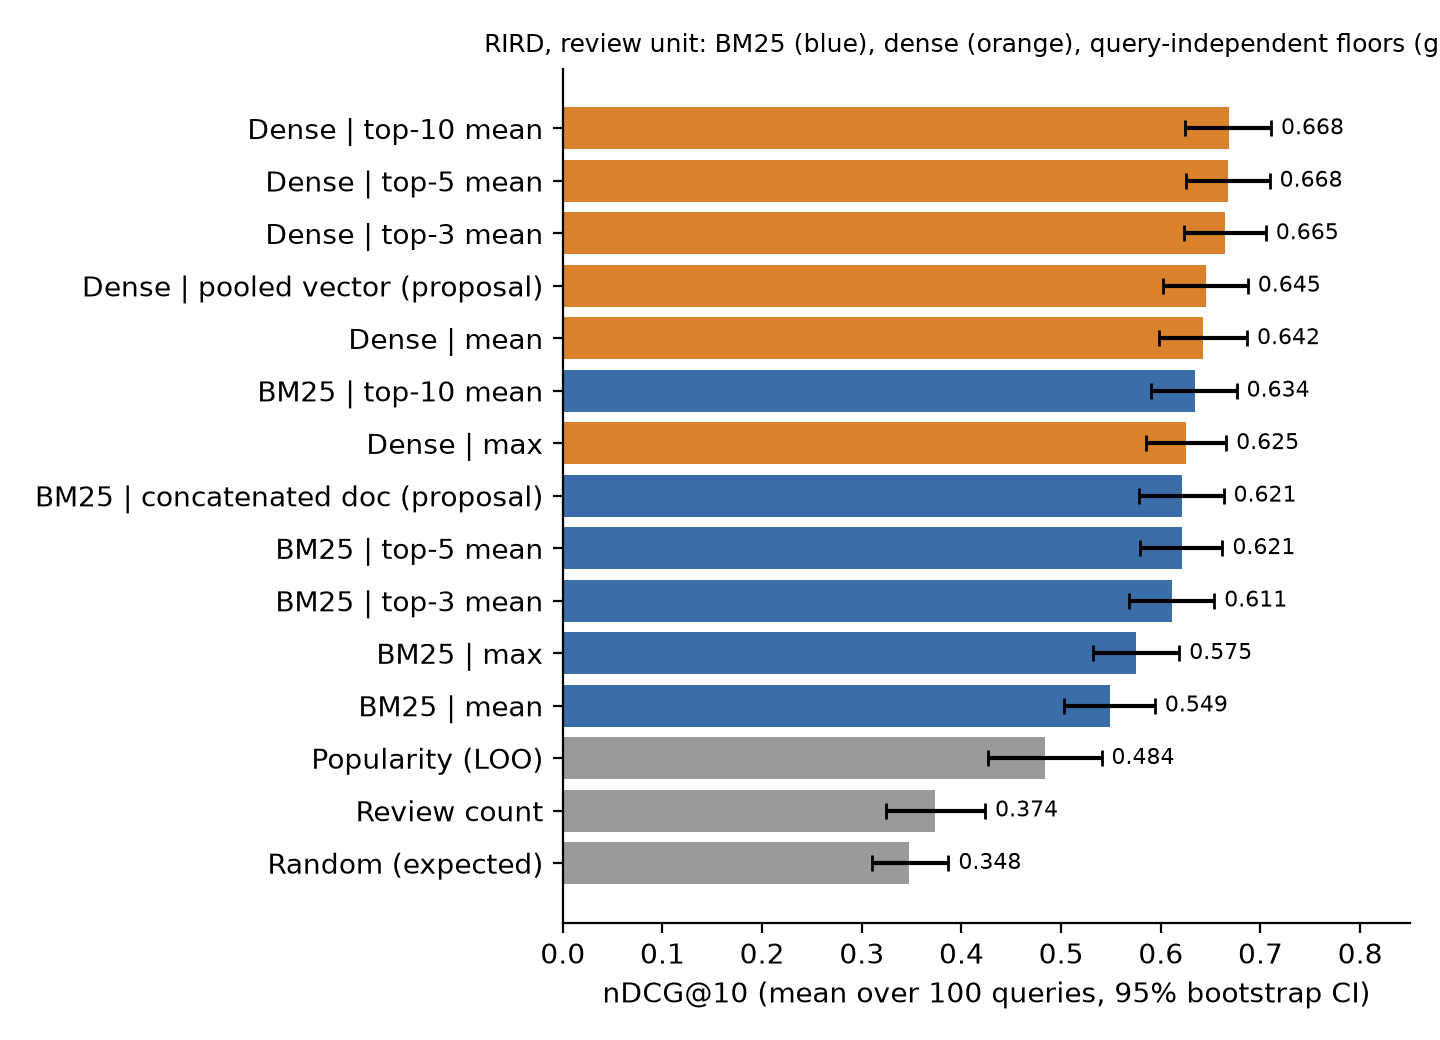
\includegraphics[width=0.88\linewidth]{figures/v2_ndcg_ci.png}
\caption{nDCG@10 with 95\% bootstrap CI for all review-level models and the three
query-independent floors.}
\label{fig:v2}
\end{figure}

\begin{table}[H]
\centering\small
\caption{Dense minus BM25 on the same unit and aggregation (nDCG@10), paired
randomization test, Holm-corrected over the five comparisons.}
\label{tab:sig}
\begin{tabular}{@{}lccc@{}}
\toprule
\textbf{Aggregation} & \textbf{Difference [95\% CI]} & \textbf{$p$ (Holm)} & \textbf{Significant} \\
\midrule
max         & +0.050 [0.017, 0.083] & 0.009  & yes \\
mean        & +0.094 [0.057, 0.129] & $<$0.001 & yes \\
top-3 mean  & +0.053 [0.023, 0.083] & 0.003  & yes \\
top-5 mean  & +0.047 [0.016, 0.077] & 0.009  & yes \\
top-10 mean & +0.035 [0.005, 0.063] & 0.020  & yes \\
\bottomrule
\end{tabular}
\end{table}

\noindent\textbf{Findings and interpretation.}
\begin{enumerate}
  \item \textbf{Dense beats BM25 under every aggregation}, all significant after correction
  (Table~\ref{tab:sig}). The gap is largest under mean (+0.094) and smallest under top-10 mean
  (+0.035): averaging over all reviews hurts BM25 most because most reviews share no words with
  the query and score zero, whereas cosine similarity is never exactly zero.
  \item \textbf{Top-$k$ mean is the best aggregation for both models}; max is the weakest for
  dense. One review is a noisy signal (a single enthusiastic or off-topic review can win);
  averaging the best few reviews keeps the focus on query-relevant evidence while smoothing
  that noise.
  \item \textbf{Everything except BM25 mean beats the popularity floor} (BM25 mean: +0.065,
  Holm $p = 0.056$). Popularity alone already reaches nDCG@10 0.484, so a large part of
  ``accuracy'' on RIRD is knowing which restaurants are relevant to many queries.
  \item \textbf{Negative result: the fair setup did not significantly improve on the proposal
  baselines.} Dense top-10 mean is +0.023 over the proposal's pooled vector, but not
  significant (Holm $p = 0.64$), and BM25 mean is significantly \emph{worse} than the
  proposal's concatenated document ($-0.072$). The point of the revision is a fair
  comparison, not a higher number; the proposal's
  conclusion (dense $>$ BM25) survives the fix.
  \item \textbf{Context.} Off-the-shelf dense with top-10 mean reaches MAP 0.608, close to
  the 0.626 of the fine-tuned model in \citet{rird2023}. These are different encoders and
  training regimes, so this is not a like-for-like comparison, but it shows that a
  multilingual encoder used without training is a reasonable base for both languages.
\end{enumerate}

\section{Review-Volume Control}
\label{sec:res-a3}
\begin{figure}[H]
\centering
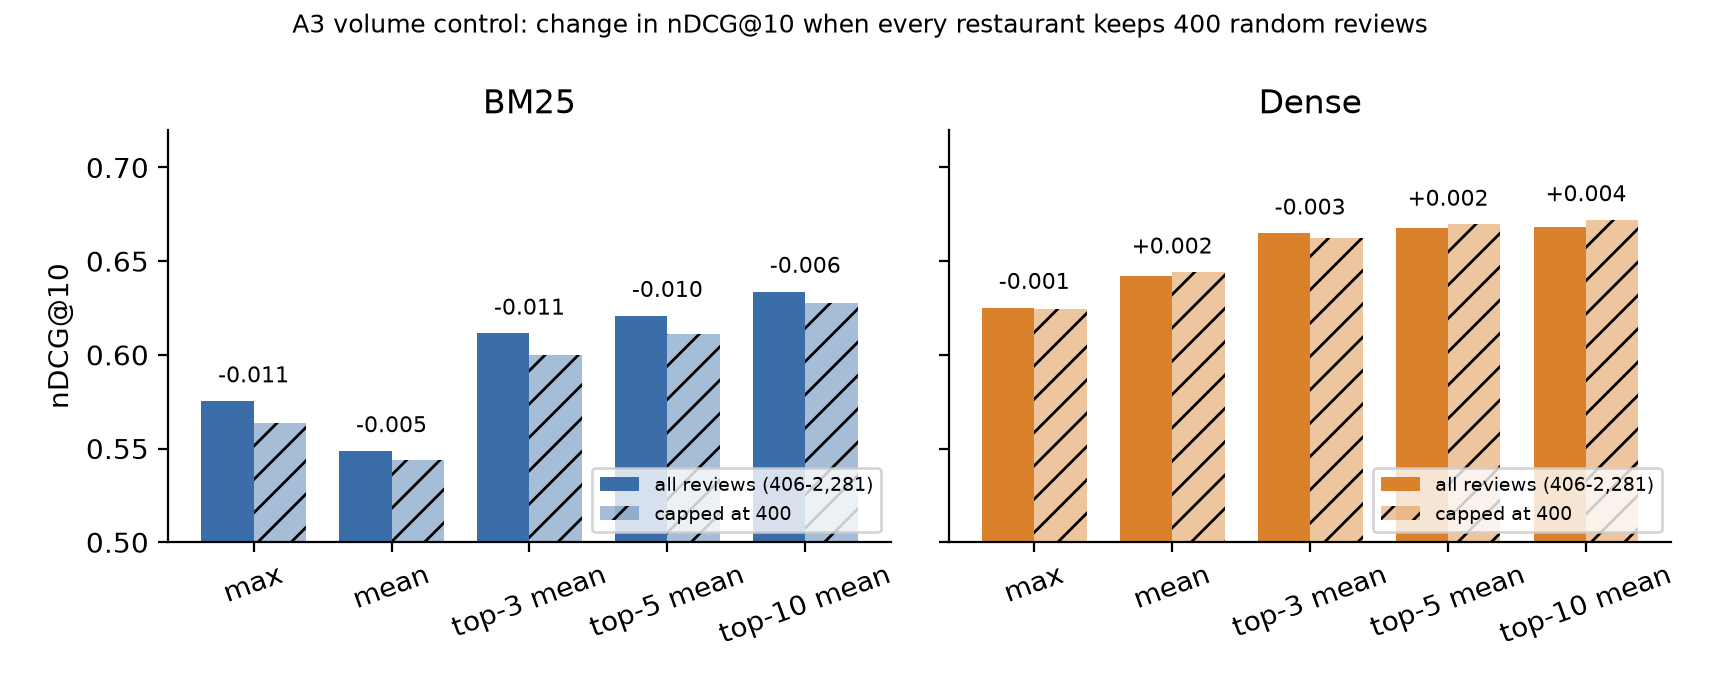
\includegraphics[width=\linewidth]{figures/a3_volume_control.png}
\caption{nDCG@10 with all reviews versus 400 randomly sampled reviews per restaurant. Labels
give the change.}
\label{fig:a3}
\end{figure}

\begin{table}[H]
\centering\small
\caption{Correlation between restaurant score and review count, averaged over the 100
queries (Pearson / Spearman). ``Capped'' correlates the capped scores with the original
counts.}
\label{tab:a3corr}
\begin{tabular}{@{}lcccc@{}}
\toprule
& \multicolumn{2}{c}{\textbf{BM25}} & \multicolumn{2}{c}{\textbf{Dense}} \\
\cmidrule(lr){2-3}\cmidrule(lr){4-5}
\textbf{Aggregation} & \textbf{all reviews} & \textbf{capped} & \textbf{all reviews} & \textbf{capped} \\
\midrule
max         & 0.21 / 0.18 & 0.01 / 0.00 & 0.22 / 0.11 & 0.03 / $-$0.04 \\
mean        & $-$0.05 / $-$0.06 & $-$0.07 / $-$0.07 & 0.04 / $-$0.06 & 0.03 / $-$0.06 \\
top-3 mean  & 0.28 / 0.23 & 0.00 / $-$0.01 & 0.26 / 0.14 & 0.04 / $-$0.04 \\
top-5 mean  & 0.31 / 0.26 & 0.00 / $-$0.01 & 0.28 / 0.15 & 0.04 / $-$0.05 \\
top-10 mean & 0.36 / 0.30 & $-$0.01 / $-$0.02 & 0.30 / 0.16 & 0.04 / $-$0.05 \\
\bottomrule
\end{tabular}
\end{table}

\noindent\textbf{Findings and interpretation.}
\begin{enumerate}
  \item \textbf{The predicted bias exists.} Within a query, max and top-$k$ scores rise with
  review count (Pearson 0.21--0.36), while the mean shows none, exactly as the ``more chances''
  argument in Section~\ref{sec:f2} predicts. Capping removes it.
  \item \textbf{It does not change accuracy or conclusions.} Dense moves by at most $\pm$0.004
  nDCG@10; BM25 loses 0.005--0.011; dense stays best under every aggregation.
  \item \textbf{Part of the bias is signal, not noise.} Restaurants with more reviews are
  relevant to more queries (Spearman 0.30 between review count and number of relevant queries
  over the 50 restaurants). BM25's small loss when capped is consistent with removing some
  genuine evidence: BM25 needs exact word matches, and fewer reviews means fewer matches.
  \item \textbf{A lesson about measurement.} Pooling all queries into one correlation gave
  only 0.05--0.12, because score scales differ between queries; the per-query average shows
  the real effect. We report the per-query version.
  \item \textbf{Limits.} One sampling seed; no paired test between the full and capped runs
  yet; RIRD only contains restaurants with at least 400 reviews, so smaller restaurants (where
  volume effects would be stronger) are not represented.
\end{enumerate}

\section{First Look at the Explanations}
\label{sec:res-expl}
The two explanation tests have not been run yet, but the saved evidence lets us inspect what
the system currently shows. Table~\ref{tab:expl} gives the top evidence for two queries under the best model.

\begin{table}[H]
\centering\small
\caption{Top evidence review for the two highest-ranked restaurants (dense, top-10 mean).
``Relevant'' is the RIRD label.}
\label{tab:expl}
\begin{tabularx}{\textwidth}{@{}p{2.3cm}p{3.4cm}cL@{}}
\toprule
\textbf{Query} & \textbf{Rank: restaurant} & \textbf{Relevant} & \textbf{Top evidence (excerpt)} \\
\midrule
I am on a budget & 1: Fishman Lobster Clubhouse & no & ``It's not bad but kinda pricey.'' \\
 & 2: Dragon Boat Fusion & yes & ``Good dim sum, pretty standard prices/service.'' \\
\midrule
Non-spicy Chinese meals & 1: Ding Tai Fung & yes & 94-word review on Northern Chinese food (\ldots) ``they use a lot of oil'' \\
 & & & 2nd evidence: ``\ldots Wonton was spicy \ldots red chili oil'' \\
 & 2: Pai Northern Thai Kitchen & no & ``Perfect Thai Curry in nice easy going atmosphere \ldots'' \\
\bottomrule
\end{tabularx}
\end{table}

\noindent\textbf{What this shows.}
\begin{itemize}
  \item \textbf{Topic match without support.} The dense model matches the \emph{topic} of the
  query (price, spiciness, Asian food) but not its \emph{polarity}: a review saying a place
  is pricey ranks a restaurant first for ``I am on a budget''; a sentence saying the wonton
  was spicy is shown for ``non-spicy''. These are exactly the cases the professor warned
  about: relevant-looking, faithful to the model, but not supporting.
  \item \textbf{Whole reviews are too coarse to be explanations.} A 94-word review mixes
  several aspects, and the part that supports the query cannot be told apart from the rest.
  This motivates the sentence-level rerun before the human rating.
  \item \textbf{Prediction.} We expect a clear share of shown evidence to be rated 0 for
  negation and price queries; the support rating will measure how large it is.
\end{itemize}

\section{Thai Sentence Retrieval (RQ3, Qualitative)}
\label{sec:res-thai}
\textbf{Segmentation spot-check} (2,000-review pilot, 19,294 sentences, 9.6 per review;
checked by a native speaker). Short, informal reviews (most of Wongnai) split cleanly. Two
error patterns: cuts after abbreviation dots such as \thai{กทม.} and \thai{ม.ค.} (0.7\% of
sentences) and long blog-style sections merged into one sentence (1.6\% over 200 characters).
Taste statements such as \thai{เผ็ดมาก} or \thai{ไม่หวานมาก} are short and almost always survive
intact. We judge segmentation good enough for retrieval and report \texttt{crfcut}'s published
accuracy on review text as a limitation \citep{lowphansirikul2020scb}.

\begin{table}[H]
\centering\small
\caption{Top-3 Thai sentences for one query of each type (2,000-review pilot, inspected but not
yet labelled).}
\label{tab:thai}
\begin{tabularx}{\textwidth}{@{}>{\raggedright\arraybackslash}p{3.3cm}LL@{}}
\toprule
\textbf{Query} & \textbf{BM25} & \textbf{Dense} \\
\midrule
T02 \thai{อยากกินอะไรเผ็ดๆ แบบจัดๆ} (really spicy) &
\thai{เนื่องจากอยากกินปูเน้นๆเนื้อๆ เลยจัดเต็ม}\newline
\thai{อยากกินอะไรเบาๆและชิมชานมเย็น}\newline
\thai{ถ้าอยากกินไอติมแบบอร่อย นั่งคุยกันสบายๆ} &
\thai{ถ้าชอบเผ็ดสั่งเพิ่มได้เลย}\newline
\thai{สำหรับคนชอบเผ็ดๆเลย}\newline
\thai{ต้องกินกับซอสที่ออกเปรี้ยวๆ แซลมอนรมควัน} \\
\midrule
T11 \thai{ต้มยำเปรี้ยวๆ เผ็ดๆ} (sour and spicy tom yum) &
\thai{น้ำต้มยำอร่อยๆ เปรี้ยวๆ ดี}\newline
\thai{อร่อยดี เปรี้ยวๆ เผ็ดๆ แต่ไม่เข็ดฟันเด้อ - พิซซ่าญี่ปุ่น}\newline
\thai{เปรี้ยวอย่างเดียวเปรี้ยวเผ็ดเกิน} &
\thai{เผ็ดเปรี้ยวนำ - ลาบหมู}\newline
\thai{น้ำต้มยำเปรี้ยวแซ่บ หอมกลิ่นพริกขี้หนู}\newline
\thai{ยำหมูยอแซ่บซี้ด} \\
\midrule
T20 \thai{ของหวานที่ไม่หวานมาก} (desserts not too sweet) &
\thai{ตอบโจทย์วัยรุ่นที่อยากกินของหวานแต่ไม่ชอบแบบหวานเลี่ยน}\newline
\thai{ไม่หวานมากอย่างที่คิดไว้}\newline
\thai{ไม่หวานมากกำลังดี} &
\thai{และมีความหวานน้อย}\newline
\thai{ขนมถ้วย : ไม่หวานมาก}\newline
\thai{ไม่หวานมากแล้วก็ไม่ฝาดมาก ปล.} \\
\bottomrule
\end{tabularx}
\end{table}

\noindent\textbf{Observations (to be confirmed by labels).}
\begin{itemize}
  \item \textbf{BM25 is fooled by filler words.} For T02 it matches \thai{อยากกินอะไร}
  (``want to eat something'') and \thai{จัด}, not spiciness. Dense finds spicy sentences.
  \item \textbf{Dense drifts by topic.} For T11 it returns sour-spicy sentences about other
  dishes (larb, yam); for T02 its fifth result describes the opposite taste
  (\thai{รสชาติจะออกอ่อนๆ}, ``mild'').
  \item \textbf{Both handle the T20 negation}, unlike English findings on negation
  \citep{weller2024nevir}. A possible reason is that BM25 keeps \thai{ไม่} as a token and the
  phrase \thai{ไม่หวานมาก} is common in Thai reviews; this is a hypothesis for the labelled
  results.
  \item \textbf{The two systems are complementary.} Their top-10 lists share fewer than one
  sentence per query on average, so pooling them roughly doubles what must be labelled
  (465 pairs in the pilot) but makes the comparison informative.
\end{itemize}

\section{Challenges}
\begin{itemize}
  \item \textbf{Review truncation.} 19.9\% of RIRD reviews exceed the encoder's 256-token
  limit (50.6\% exceeded the 128 tokens used in the proposal), so part of each long review is never
  seen by the dense model. This is a further reason for the sentence unit.
  \item \textbf{Thai labels need native speakers.} Relevance in Thai can only be judged by a
  native speaker, and a second independent annotator is needed for the agreement check.
  \item \textbf{Small Thai test set.} With 24 queries, only nDCG@10 differences of roughly
  0.11--0.17 can be detected reliably; a non-significant result will be reported as ``no
  evidence of a difference'', not as ``equal''.
\end{itemize}

\FloatBarrier

% =====================================================================
%  CHAPTER 6: NEXT STEPS
% =====================================================================
\chapter{Remaining Work and Plan}
\label{ch:next}

\section{Remaining Tasks}
\begin{table}[H]
\centering\small
\caption{Remaining work and target weeks after the progress presentation
(week 1 starts 21 October 2026).}
\label{tab:plan}
\begin{tabularx}{\textwidth}{@{}p{3.4cm}Lp{1.1cm}@{}}
\toprule
\textbf{Work item} & \textbf{Description} & \textbf{Week} \\
\midrule
Sentence-level rerun & Repeat the full RIRD comparison with sentences as the unit; repeat the volume control with more seeds and a paired test & 1 \\
Thai pool & Run retrieval on the 10,000-review corpus and build the blind labelling sheet & 1 \\
Guidelines & Final native-speaker review of the annotation guidelines & 1 \\
Deletion test & Faithfulness at sentence level, $m\in\{1,3,5,10\}$, versus random deletion & 2 \\
Thai labelling & Label the pooled sentences (about 450 pairs) & 2 \\
Support rating & 270 explanation items rated independently by two annotators; kappa & 3 \\
Thai agreement & Second native speaker labels 60 pairs; kappa & 3 \\
Thai scores & nDCG@10 and P@10 for BM25 vs dense, by query type & 3 \\
Final write-up & Final claims, report, slides and video & 4 \\
\bottomrule
\end{tabularx}
\end{table}

\section{Expected Outcome and Fallbacks}
\begin{itemize}
  \item \textbf{RQ1} will be answered at both review and sentence level, with the volume
  control. We expect dense to remain ahead; whether the sentence unit helps is open.
  \item \textbf{RQ2} will give two numbers per model: the rank drop caused by deleting the
  shown evidence (versus random) and the share of shown sentences that people rate as
  supporting, with kappa. A low support rate would be a valid, reportable negative finding.
  \item \textbf{RQ3} will give Thai nDCG@10 for BM25 and dense with CIs and a negation slice.
  Based on MIRACL we do not presume a winner.
  \item \textbf{If time runs short} we reduce the Thai test set to 15 queries, then the
  support rating to 15 queries. The sentence-level rerun and the deletion test are not cut,
  because without them the final question cannot be answered.
\end{itemize}

\FloatBarrier

% =====================================================================
%  BIBLIOGRAPHY
% =====================================================================
\singlespacing
\begin{thebibliography}{99}

\bibitem[Abdollah Pour et al., 2023]{rird2023}
Abdollah Pour, M. M., Farinneya, P., Toroghi, A., Korikov, A., Pesaranghader, A.,
Sajed, T., Bharadwaj, M., Mavrin, B., \& Sanner, S. (2023). Self-supervised
contrastive BERT fine-tuning for fusion-based reviewed-item retrieval. In
\emph{Advances in Information Retrieval (ECIR 2023)}, LNCS vol.~13980 (pp.~3--17).
Springer. https://doi.org/10.1007/978-3-031-28244-7\_1

\bibitem[Balog et al., 2006]{balog2006formal}
Balog, K., Azzopardi, L., \& de Rijke, M. (2006). Formal models for expert finding in
enterprise corpora. In \emph{Proceedings of SIGIR 2006} (pp.~43--50).

\bibitem[Chen et al., 2024]{chen2024densex}
Chen, T., Wang, H., Chen, S., Yu, W., Ma, K., Zhao, X., Zhang, H., \& Yu, D. (2024). Dense X
retrieval: What retrieval granularity should we use? In \emph{Proceedings of EMNLP 2024}.
arXiv:2312.06648.

\bibitem[Cohen, 1960]{cohen1960kappa}
Cohen, J. (1960). A coefficient of agreement for nominal scales. \emph{Educational and
Psychological Measurement, 20}(1), 37--46. https://doi.org/10.1177/001316446002000104

\bibitem[DeYoung et al., 2020]{deyoung2020eraser}
DeYoung, J., Jain, S., Rajani, N. F., Lehman, E., Xiong, C., Socher, R., \& Wallace, B. C.
(2020). ERASER: A benchmark to evaluate rationalized NLP models. In \emph{Proceedings of ACL
2020} (pp.~4443--4458). https://doi.org/10.18653/v1/2020.acl-main.408

\bibitem[Hasan et al., 2025]{hasan2025reviewsurvey}
Hasan, E., Rahman, M., Ding, C., Huang, J. X., \& Raza, S. (2025). Review-based recommender
systems: A survey of approaches, challenges and future perspectives. \emph{ACM Computing
Surveys, 58}(1), 1--41. https://doi.org/10.1145/3742421

\bibitem[Highgroundbkk, n.d.]{wongnai2020}
Highgroundbkk. (n.d.). \emph{wongnai\_reviews} [Data set]. Hugging Face.
https://huggingface.co/datasets/Highgroundbkk/wongnai\_reviews

\bibitem[Jacovi \& Goldberg, 2020]{jacovi2020faithfulness}
Jacovi, A., \& Goldberg, Y. (2020). Towards faithfully interpretable NLP systems: How should
we define and evaluate faithfulness? In \emph{Proceedings of ACL 2020} (pp.~4198--4205).
https://doi.org/10.18653/v1/2020.acl-main.386

\bibitem[J{\"a}rvelin \& Kek{\"a}l{\"a}inen, 2002]{jarvelin2002ndcg}
J{\"a}rvelin, K., \& Kek{\"a}l{\"a}inen, J. (2002). Cumulated gain-based evaluation of IR
techniques. \emph{ACM Transactions on Information Systems, 20}(4), 422--446.
https://doi.org/10.1145/582415.582418

\bibitem[Korikov et al., 2024]{korikov2024multiaspect}
Korikov, A., Saad, G., Baron, E., Khan, M., Shah, M., \& Sanner, S. (2024). Multi-aspect
reviewed-item retrieval via LLM query decomposition and aspect fusion. \emph{SIGIR 2024
Workshop on Information Retrieval's Role in RAG Systems (IR-RAG)}. arXiv:2408.00878.

\bibitem[Li et al., 2021]{li2021extra}
Li, L., Zhang, Y., \& Chen, L. (2021). EXTRA: Explanation ranking datasets for explainable
recommendation. In \emph{Proceedings of SIGIR 2021}. arXiv:2102.10315.

\bibitem[Lowphansirikul et al., 2020]{lowphansirikul2020scb}
Lowphansirikul, L., Polpanumas, C., Rutherford, A. T., \& Nutanong, S. (2020).
scb-mt-en-th-2020: A large English--Thai parallel corpus. arXiv:2007.03541.

\bibitem[Macdonald \& Ounis, 2008]{macdonald2008voting}
Macdonald, C., \& Ounis, I. (2008). Voting techniques for expert search. \emph{Knowledge
and Information Systems, 16}(3), 259--280. https://doi.org/10.1007/s10115-007-0105-3

\bibitem[Phatthiyaphaibun et al., 2023]{phatthiyaphaibun2023pythainlp}
Phatthiyaphaibun, W., Chaovavanich, K., Polpanumas, C., Suriyawongkul, A., Lowphansirikul,
L., Chormai, P., Limkonchotiwat, P., Suntorntip, T., \& Udomcharoenchaikit, C. (2023).
PyThaiNLP: Thai natural language processing in Python. In \emph{Proceedings of NLP-OSS 2023}
(pp.~25--36). https://doi.org/10.18653/v1/2023.nlposs-1.4

\bibitem[Reimers \& Gurevych, 2020]{reimers2020multilingual}
Reimers, N., \& Gurevych, I. (2020). Making monolingual sentence embeddings multilingual using
knowledge distillation. In \emph{Proceedings of EMNLP 2020} (pp.~4512--4525).
https://doi.org/10.18653/v1/2020.emnlp-main.365

\bibitem[Robertson \& Zaragoza, 2009]{robertson2009bm25}
Robertson, S., \& Zaragoza, H. (2009). The probabilistic relevance framework: BM25
and beyond. \emph{Foundations and Trends in Information Retrieval, 3}(4), 333--389.
https://doi.org/10.1561/1500000019

\bibitem[Smucker et al., 2007]{smucker2007significance}
Smucker, M. D., Allan, J., \& Carterette, B. (2007). A comparison of statistical significance
tests for information retrieval evaluation. In \emph{Proceedings of CIKM 2007}
(pp.~623--632). https://doi.org/10.1145/1321440.1321528

\bibitem[Weller et al., 2024]{weller2024nevir}
Weller, O., Lawrie, D., \& Van Durme, B. (2024). NevIR: Negation in neural information
retrieval. In \emph{Proceedings of EACL 2024}. arXiv:2305.07614.

\bibitem[Zhang et al., 2023]{zhang2023miracl}
Zhang, X., Thakur, N., Ogundepo, O., Kamalloo, E., Alfonso-Hermelo, D., Li, X., Liu, Q.,
Rezagholizadeh, M., \& Lin, J. (2023). MIRACL: A multilingual retrieval dataset covering 18
diverse languages. \emph{Transactions of the ACL, 11}, 1114--1131.

\bibitem[Zhang et al., 2025]{zhang2025enhancing}
Zhang, J., Tian, Z., Feng, X., Chen, X., \& Chen, C. (2025). Enhancing recommendation
explanations through user-centric refinement. In \emph{Findings of EMNLP 2025}
(pp.~8177--8191). https://doi.org/10.18653/v1/2025.findings-emnlp.434

\end{thebibliography}

\end{document}
